\section{CAssoc\-Array\-Binding$<$ T $>$  Class Template Reference}
\label{classCAssocArrayBinding}\index{CAssocArrayBinding@{CAssoc\-Array\-Binding}}
{\tt \#include $<$CAssoc\-Array\-Binding.h$>$}

Inheritance diagram for CAssoc\-Array\-Binding$<$ T $>$::\begin{figure}[H]
\begin{center}
\leavevmode
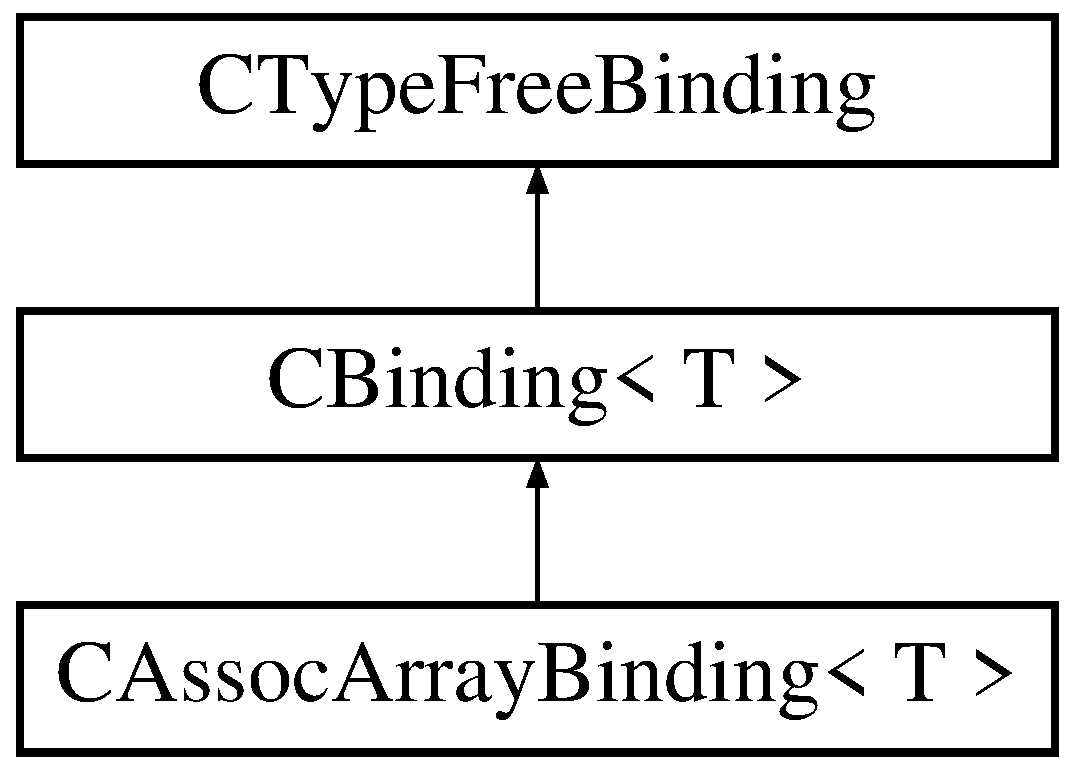
\includegraphics[height=3cm]{classCAssocArrayBinding}
\end{center}
\end{figure}
\subsection*{Public Methods}
\begin{CompactItemize}
\item 
{\bf CAssoc\-Array\-Binding} (const string \&r\-Name)
\item 
{\bf CAssoc\-Array\-Binding} (const char $\ast$p\-Name)
\item 
{\bf $\sim$CAssoc\-Array\-Binding} ()
\item 
map$<$ string, T $>$ {\bf get\-Array} () const
\begin{CompactList}\small\item\em $<$ Get entire map.\item\end{CompactList}\item 
map$<$ string, T $>$::iterator {\bf begin} ()
\item 
map$<$ string, T $>$::iterator {\bf end} ()
\item 
T \& {\bf operator[$\,$]} (const char $\ast$p\-Name)
\item 
T \& {\bf operator[$\,$]} (const string \&r\-Name)
\item 
map$<$ string, T $>$::iterator {\bf find} (const char $\ast$p\-Name)
\item 
map$<$ string, T $>$::iterator {\bf find} (const string \&r\-Name)
\item 
string {\bf get\-Name} () const
\item 
int {\bf get\-Type} () const
\item 
virtual void {\bf Init\-Bindings} ({\bf CTCLInterpreter} \&r\-Interp)
\item 
virtual void {\bf Commit} ({\bf CTCLInterpreter} \&r\-Interp)
\item 
virtual void {\bf Shutdown\-Bindings} ({\bf CTCLInterpreter} \&r\-Interp)
\item 
virtual void {\bf Dump} (int fd)
\end{CompactItemize}
\subsection*{Private Methods}
\begin{CompactItemize}
\item 
{\bf CAssoc\-Array\-Binding} (const CAssoc\-Array\-Binding \&rhs)
\item 
CAssoc\-Array\-Binding \& {\bf operator=} (const CAssoc\-Array\-Binding \&rhs)
\item 
int {\bf operator==} (const CAssoc\-Array\-Binding \&rhs)
\end{CompactItemize}
\subsection*{Private Attributes}
\begin{CompactItemize}
\item 
map$<$ string, T $>$ {\bf m\_\-Array}
\begin{CompactList}\small\item\em Data stored in this map.\item\end{CompactList}\item 
string {\bf m\_\-s\-Name}
\begin{CompactList}\small\item\em TCL Name of array.\item\end{CompactList}\item 
int {\bf m\_\-TCLVariable\-Type}
\begin{CompactList}\small\item\em Type of data in the array.\item\end{CompactList}\end{CompactItemize}


\subsection{Detailed Description}
\subsubsection*{template$<$class T$>$ class CAssoc\-Array\-Binding$<$ T $>$}

Encapsulates the configuration of an associative array. Associative arrays are arrays whose indices are strings rather than numbers. One use of associative arrays is to provide meaningful subscripts to configuration items. For example, suppose I want to store the thresholds for all of my 'detector' adc's. I might have an associative array named thresholds with subscripts which indicate detector segment and  subtype e.g. \char`\"{}seg1,de\char`\"{} could be an index. Some key properties of  associative arrays:\begin{CompactItemize}
\item 
One can iterate through the elements which have been given a value\item 
One can index by subscript, however if the element does not yet exist, it will be generated and the value will be that provided by the default constructor. Note that this is a null pointer for characters.\item 
There is no way to provide default values to elements in this clas. \end{CompactItemize}




Definition at line 326 of file CAssoc\-Array\-Binding.h.

\subsection{Constructor \& Destructor Documentation}
\index{CAssocArrayBinding@{CAssoc\-Array\-Binding}!CAssocArrayBinding@{CAssocArrayBinding}}
\index{CAssocArrayBinding@{CAssocArrayBinding}!CAssocArrayBinding@{CAssoc\-Array\-Binding}}
\subsubsection{\setlength{\rightskip}{0pt plus 5cm}template$<$class T$>$ CAssoc\-Array\-Binding$<$ T $>$::CAssoc\-Array\-Binding (const string \& {\em r\-Name})}\label{classCAssocArrayBinding_a0}


Constructs an associative array configured from a TCL array. The TCL array name is specified by a const string\& \begin{Desc}
\item[Parameters: ]\par
\begin{description}
\item[{\em 
r\-Name}]- Name of the configuration array. \end{description}
\end{Desc}


Definition at line 309 of file CAssoc\-Array\-Binding.cpp.

References CAssoc\-Array\-Binding$<$ T $>$::m\_\-TCLVariable\-Type, and CBinding$<$ T $>$::Variable\-Type().\index{CAssocArrayBinding@{CAssoc\-Array\-Binding}!CAssocArrayBinding@{CAssocArrayBinding}}
\index{CAssocArrayBinding@{CAssocArrayBinding}!CAssocArrayBinding@{CAssoc\-Array\-Binding}}
\subsubsection{\setlength{\rightskip}{0pt plus 5cm}template$<$class T$>$ CAssoc\-Array\-Binding$<$ T $>$::CAssoc\-Array\-Binding (const char $\ast$ {\em p\-Name})}\label{classCAssocArrayBinding_a1}


Constructs an associative array configured from a TCL array. The TCL array name is speicified by a const char$\ast$ \begin{Desc}
\item[Parameters: ]\par
\begin{description}
\item[{\em 
p\-Name}]- Name of the configuration array. \end{description}
\end{Desc}


Definition at line 322 of file CAssoc\-Array\-Binding.cpp.

References CAssoc\-Array\-Binding$<$ T $>$::m\_\-TCLVariable\-Type, and CBinding$<$ T $>$::Variable\-Type().\index{CAssocArrayBinding@{CAssoc\-Array\-Binding}!~CAssocArrayBinding@{$\sim$CAssocArrayBinding}}
\index{~CAssocArrayBinding@{$\sim$CAssocArrayBinding}!CAssocArrayBinding@{CAssoc\-Array\-Binding}}
\subsubsection{\setlength{\rightskip}{0pt plus 5cm}template$<$class T$>$ CAssoc\-Array\-Binding$<$ T $>$::$\sim$CAssoc\-Array\-Binding ()}\label{classCAssocArrayBinding_a2}


The destructor will need to delete storage associated with character entries in the map. 

Definition at line 334 of file CAssoc\-Array\-Binding.cpp.

References CAssoc\-Array\-Binding$<$ T $>$::m\_\-Array, and CAssoc\-Array\-Binding$<$ T $>$::m\_\-TCLVariable\-Type.\index{CAssocArrayBinding@{CAssoc\-Array\-Binding}!CAssocArrayBinding@{CAssocArrayBinding}}
\index{CAssocArrayBinding@{CAssocArrayBinding}!CAssocArrayBinding@{CAssoc\-Array\-Binding}}
\subsubsection{\setlength{\rightskip}{0pt plus 5cm}template$<$class T$>$ CAssoc\-Array\-Binding$<$ T $>$::CAssoc\-Array\-Binding (const CAssoc\-Array\-Binding$<$ T $>$ \& {\em rhs})\hspace{0.3cm}{\tt  [private]}}\label{classCAssocArrayBinding_c0}




\subsection{Member Function Documentation}
\index{CAssocArrayBinding@{CAssoc\-Array\-Binding}!begin@{begin}}
\index{begin@{begin}!CAssocArrayBinding@{CAssoc\-Array\-Binding}}
\subsubsection{\setlength{\rightskip}{0pt plus 5cm}template$<$class T$>$ map$<$string,T$>$::iterator CAssoc\-Array\-Binding$<$ T $>$::begin ()\hspace{0.3cm}{\tt  [inline]}}\label{classCAssocArrayBinding_a4}




Definition at line 350 of file CAssoc\-Array\-Binding.h.

References CAssoc\-Array\-Binding$<$ T $>$::m\_\-Array.\index{CAssocArrayBinding@{CAssoc\-Array\-Binding}!Commit@{Commit}}
\index{Commit@{Commit}!CAssocArrayBinding@{CAssoc\-Array\-Binding}}
\subsubsection{\setlength{\rightskip}{0pt plus 5cm}template$<$class T$>$ void CAssoc\-Array\-Binding$<$ T $>$::Commit ({\bf CTCLInterpreter} \& {\em r\-Interp})\hspace{0.3cm}{\tt  [virtual]}}\label{classCAssocArrayBinding_a13}


Commits the bindings to the array. In this case we will determine the set of indices the variable has (by running a string script of the form \char`\"{}array names m\_\-s\-Name\char`\"{}, and fetching the results from the result string. For each item in the TCL array an item is created in the  m\_\-Array. Note that if the type is TCL\_\-BIND\_\-STRING, dynamic memory is allocated to hold the result string. \begin{Desc}
\item[Parameters: ]\par
\begin{description}
\item[{\em 
r\-Interp}]- the interpreter which read in the config file. Used to fetch variable strings etc. \end{description}
\end{Desc}


Implements {\bf CBinding$<$ T $>$} {\rm (p.\,\pageref{classCBinding_a1})}.

Definition at line 371 of file CAssoc\-Array\-Binding.cpp.

References CTCLInterpreter::Expr\-Boolean(), CTCLInterpreter::Expr\-Double(), CTCLInterpreter::Expr\-Long(), CTCLInterpreter::get\-Interpreter(), CTCLInterpreter::Global\-Eval(), CAssoc\-Array\-Binding$<$ T $>$::m\_\-Array, CAssoc\-Array\-Binding$<$ T $>$::m\_\-s\-Name, CTCLList::Split(), and String\-Array.\index{CAssocArrayBinding@{CAssoc\-Array\-Binding}!Dump@{Dump}}
\index{Dump@{Dump}!CAssocArrayBinding@{CAssoc\-Array\-Binding}}
\subsubsection{\setlength{\rightskip}{0pt plus 5cm}template$<$class T$>$ void CAssoc\-Array\-Binding$<$ T $>$::Dump (int {\em fd})\hspace{0.3cm}{\tt  [virtual]}}\label{classCAssocArrayBinding_a15}


Dumps the contents of the array out in a form which allows the array to be recovered by reading the file. \begin{Desc}
\item[Parameters: ]\par
\begin{description}
\item[{\em 
fd}]- A file descriptor on which to write this data. \end{description}
\end{Desc}


Implements {\bf CBinding$<$ T $>$} {\rm (p.\,\pageref{classCBinding_a2})}.

Definition at line 469 of file CAssoc\-Array\-Binding.cpp.

References CBinding$<$ T $>$::Item\-To\-String(), CAssoc\-Array\-Binding$<$ T $>$::m\_\-Array, and CAssoc\-Array\-Binding$<$ T $>$::m\_\-s\-Name.\index{CAssocArrayBinding@{CAssoc\-Array\-Binding}!end@{end}}
\index{end@{end}!CAssocArrayBinding@{CAssoc\-Array\-Binding}}
\subsubsection{\setlength{\rightskip}{0pt plus 5cm}template$<$class T$>$ map$<$string,T$>$::iterator CAssoc\-Array\-Binding$<$ T $>$::end ()\hspace{0.3cm}{\tt  [inline]}}\label{classCAssocArrayBinding_a5}




Definition at line 353 of file CAssoc\-Array\-Binding.h.

References CAssoc\-Array\-Binding$<$ T $>$::m\_\-Array.\index{CAssocArrayBinding@{CAssoc\-Array\-Binding}!find@{find}}
\index{find@{find}!CAssocArrayBinding@{CAssoc\-Array\-Binding}}
\subsubsection{\setlength{\rightskip}{0pt plus 5cm}template$<$class T$>$ map$<$string,T$>$::iterator CAssoc\-Array\-Binding$<$ T $>$::find (const string \& {\em r\-Name})\hspace{0.3cm}{\tt  [inline]}}\label{classCAssocArrayBinding_a9}




Definition at line 366 of file CAssoc\-Array\-Binding.h.

References CAssoc\-Array\-Binding$<$ T $>$::m\_\-Array.\index{CAssocArrayBinding@{CAssoc\-Array\-Binding}!find@{find}}
\index{find@{find}!CAssocArrayBinding@{CAssoc\-Array\-Binding}}
\subsubsection{\setlength{\rightskip}{0pt plus 5cm}template$<$class T$>$ map$<$string,T$>$::iterator CAssoc\-Array\-Binding$<$ T $>$::find (const char $\ast$ {\em p\-Name})\hspace{0.3cm}{\tt  [inline]}}\label{classCAssocArrayBinding_a8}




Definition at line 363 of file CAssoc\-Array\-Binding.h.

References CAssoc\-Array\-Binding$<$ T $>$::m\_\-Array.\index{CAssocArrayBinding@{CAssoc\-Array\-Binding}!getArray@{getArray}}
\index{getArray@{getArray}!CAssocArrayBinding@{CAssoc\-Array\-Binding}}
\subsubsection{\setlength{\rightskip}{0pt plus 5cm}template$<$class T$>$ map$<$string,T$>$ CAssoc\-Array\-Binding$<$ T $>$::get\-Array () const\hspace{0.3cm}{\tt  [inline]}}\label{classCAssocArrayBinding_a3}


$<$ Get entire map.



Definition at line 346 of file CAssoc\-Array\-Binding.h.

References CAssoc\-Array\-Binding$<$ T $>$::m\_\-Array.\index{CAssocArrayBinding@{CAssoc\-Array\-Binding}!getName@{getName}}
\index{getName@{getName}!CAssocArrayBinding@{CAssoc\-Array\-Binding}}
\subsubsection{\setlength{\rightskip}{0pt plus 5cm}template$<$class T$>$ string CAssoc\-Array\-Binding$<$ T $>$::get\-Name () const\hspace{0.3cm}{\tt  [inline]}}\label{classCAssocArrayBinding_a10}




Definition at line 370 of file CAssoc\-Array\-Binding.h.

References CAssoc\-Array\-Binding$<$ T $>$::m\_\-s\-Name.\index{CAssocArrayBinding@{CAssoc\-Array\-Binding}!getType@{getType}}
\index{getType@{getType}!CAssocArrayBinding@{CAssoc\-Array\-Binding}}
\subsubsection{\setlength{\rightskip}{0pt plus 5cm}template$<$class T$>$ int CAssoc\-Array\-Binding$<$ T $>$::get\-Type () const\hspace{0.3cm}{\tt  [inline]}}\label{classCAssocArrayBinding_a11}




Definition at line 374 of file CAssoc\-Array\-Binding.h.

References CAssoc\-Array\-Binding$<$ T $>$::m\_\-TCLVariable\-Type.\index{CAssocArrayBinding@{CAssoc\-Array\-Binding}!InitBindings@{InitBindings}}
\index{InitBindings@{InitBindings}!CAssocArrayBinding@{CAssoc\-Array\-Binding}}
\subsubsection{\setlength{\rightskip}{0pt plus 5cm}template$<$class T$>$ void CAssoc\-Array\-Binding$<$ T $>$::Init\-Bindings ({\bf CTCLInterpreter} \& {\em r\-Interp})\hspace{0.3cm}{\tt  [virtual]}}\label{classCAssocArrayBinding_a12}


Initialize the bindings prior to reading in the configuration file. for this class the actual binding operation is done in the commit phase so this is a no-op. \begin{Desc}
\item[Parameters: ]\par
\begin{description}
\item[{\em 
r\-Interp}]- Referencers the TCL interpreter which will be used to read in the configuration file. \end{description}
\end{Desc}


Implements {\bf CBinding$<$ T $>$} {\rm (p.\,\pageref{classCBinding_a0})}.

Definition at line 354 of file CAssoc\-Array\-Binding.cpp.\index{CAssocArrayBinding@{CAssoc\-Array\-Binding}!operator=@{operator=}}
\index{operator=@{operator=}!CAssocArrayBinding@{CAssoc\-Array\-Binding}}
\subsubsection{\setlength{\rightskip}{0pt plus 5cm}template$<$class T$>$ CAssoc\-Array\-Binding\& CAssoc\-Array\-Binding$<$ T $>$::operator= (const CAssoc\-Array\-Binding$<$ T $>$ \& {\em rhs})\hspace{0.3cm}{\tt  [private]}}\label{classCAssocArrayBinding_c1}


\index{CAssocArrayBinding@{CAssoc\-Array\-Binding}!operator==@{operator==}}
\index{operator==@{operator==}!CAssocArrayBinding@{CAssoc\-Array\-Binding}}
\subsubsection{\setlength{\rightskip}{0pt plus 5cm}template$<$class T$>$ int CAssoc\-Array\-Binding$<$ T $>$::operator== (const CAssoc\-Array\-Binding$<$ T $>$ \& {\em rhs})\hspace{0.3cm}{\tt  [private]}}\label{classCAssocArrayBinding_c2}


\index{CAssocArrayBinding@{CAssoc\-Array\-Binding}!operator[]@{operator[]}}
\index{operator[]@{operator[]}!CAssocArrayBinding@{CAssoc\-Array\-Binding}}
\subsubsection{\setlength{\rightskip}{0pt plus 5cm}template$<$class T$>$ T\& CAssoc\-Array\-Binding$<$ T $>$::operator[$\,$] (const string \& {\em r\-Name})\hspace{0.3cm}{\tt  [inline]}}\label{classCAssocArrayBinding_a7}




Definition at line 360 of file CAssoc\-Array\-Binding.h.

References CAssoc\-Array\-Binding$<$ T $>$::m\_\-Array.\index{CAssocArrayBinding@{CAssoc\-Array\-Binding}!operator[]@{operator[]}}
\index{operator[]@{operator[]}!CAssocArrayBinding@{CAssoc\-Array\-Binding}}
\subsubsection{\setlength{\rightskip}{0pt plus 5cm}template$<$class T$>$ T\& CAssoc\-Array\-Binding$<$ T $>$::operator[$\,$] (const char $\ast$ {\em p\-Name})\hspace{0.3cm}{\tt  [inline]}}\label{classCAssocArrayBinding_a6}




Definition at line 356 of file CAssoc\-Array\-Binding.h.

References CAssoc\-Array\-Binding$<$ T $>$::m\_\-Array.\index{CAssocArrayBinding@{CAssoc\-Array\-Binding}!ShutdownBindings@{ShutdownBindings}}
\index{ShutdownBindings@{ShutdownBindings}!CAssocArrayBinding@{CAssoc\-Array\-Binding}}
\subsubsection{\setlength{\rightskip}{0pt plus 5cm}template$<$class T$>$ void CAssoc\-Array\-Binding$<$ T $>$::Shutdown\-Bindings ({\bf CTCLInterpreter} \& {\em r\-Interp})\hspace{0.3cm}{\tt  [virtual]}}\label{classCAssocArrayBinding_a14}


Closes out whatever needs closing prior to deleting the interpreter which was used to read the configuration file. In this case, no action is taken as the 'binding' is done at commit time and no real connection is made between the interpreter and the array. \begin{Desc}
\item[Parameters: ]\par
\begin{description}
\item[{\em 
r\-Interp}]- Interpreter which read the config file. \end{description}
\end{Desc}


Implements {\bf CType\-Free\-Binding} {\rm (p.\,\pageref{classCTypeFreeBinding_a2})}.

Definition at line 459 of file CAssoc\-Array\-Binding.cpp.

\subsection{Member Data Documentation}
\index{CAssocArrayBinding@{CAssoc\-Array\-Binding}!m_Array@{m\_\-Array}}
\index{m_Array@{m\_\-Array}!CAssocArrayBinding@{CAssoc\-Array\-Binding}}
\subsubsection{\setlength{\rightskip}{0pt plus 5cm}template$<$class T$>$ map$<$string,T$>$ CAssoc\-Array\-Binding$<$ T $>$::m\_\-Array\hspace{0.3cm}{\tt  [private]}}\label{classCAssocArrayBinding_o0}


Data stored in this map.



Definition at line 330 of file CAssoc\-Array\-Binding.h.

Referenced by CAssoc\-Array\-Binding$<$ T $>$::begin(), CAssoc\-Array\-Binding$<$ T $>$::Commit(), CAssoc\-Array\-Binding$<$ T $>$::Dump(), CAssoc\-Array\-Binding$<$ T $>$::end(), CAssoc\-Array\-Binding$<$ T $>$::find(), CAssoc\-Array\-Binding$<$ T $>$::get\-Array(), CAssoc\-Array\-Binding$<$ T $>$::operator[$\,$](), and CAssoc\-Array\-Binding$<$ T $>$::$\sim$CAssoc\-Array\-Binding().\index{CAssocArrayBinding@{CAssoc\-Array\-Binding}!m_sName@{m\_\-sName}}
\index{m_sName@{m\_\-sName}!CAssocArrayBinding@{CAssoc\-Array\-Binding}}
\subsubsection{\setlength{\rightskip}{0pt plus 5cm}template$<$class T$>$ string CAssoc\-Array\-Binding$<$ T $>$::m\_\-s\-Name\hspace{0.3cm}{\tt  [private]}}\label{classCAssocArrayBinding_o1}


TCL Name of array.



Definition at line 331 of file CAssoc\-Array\-Binding.h.

Referenced by CAssoc\-Array\-Binding$<$ T $>$::Commit(), CAssoc\-Array\-Binding$<$ T $>$::Dump(), and CAssoc\-Array\-Binding$<$ T $>$::get\-Name().\index{CAssocArrayBinding@{CAssoc\-Array\-Binding}!m_TCLVariableType@{m\_\-TCLVariableType}}
\index{m_TCLVariableType@{m\_\-TCLVariableType}!CAssocArrayBinding@{CAssoc\-Array\-Binding}}
\subsubsection{\setlength{\rightskip}{0pt plus 5cm}template$<$class T$>$ int CAssoc\-Array\-Binding$<$ T $>$::m\_\-TCLVariable\-Type\hspace{0.3cm}{\tt  [private]}}\label{classCAssocArrayBinding_o2}


Type of data in the array.



Definition at line 332 of file CAssoc\-Array\-Binding.h.

Referenced by CAssoc\-Array\-Binding$<$ T $>$::CAssoc\-Array\-Binding(), CAssoc\-Array\-Binding$<$ T $>$::get\-Type(), and CAssoc\-Array\-Binding$<$ T $>$::$\sim$CAssoc\-Array\-Binding().

The documentation for this class was generated from the following files:\begin{CompactItemize}
\item 
{\bf CAssoc\-Array\-Binding.h}\item 
{\bf CAssoc\-Array\-Binding.cpp}\end{CompactItemize}
